\section{Практическая часть}
\subsection{Исходные данные для расчета}
Концентрация отбора $c_{P} =$ \var{concentraion_product};

Концентрация питания $c_{F} =$ \var{concentraion_feed};

Концентрация отвала $c_{W} =$ \var{concentraion_waste};

Температура $T =$ \var{temperature} $^{o}C$;

Поток отбора $P =$ \var{product_flow} $\dfrac{\text{кг}}{\text{год}}$;

Доля сокращения потока на одной ТТ $r =$ \var{flow_reduction_share} \%;

Количество ТТ в одной колонне $N =$ \var{number_theoretical_plates}.
\subsection{Расчет изменения изотопной концентрации по каскаду в 
стационарном режиме}
Поток отбора переведен из кг/год в моль/ч:

$P = \var{product_flow} \dfrac{\text{кг}}{\text{год}} = \dfrac{\var{product_flow} \dfrac{\text{кг}}{\text{год}}}{M} 
= \dfrac{\var{product_flow}\cdot\dfrac{1}{365\cdot 24} \dfrac{\text{кг}}{\text{ч}}}
{(7c_{P}+6(1-c_{P}))\cdot 10^{-3} \dfrac{\text{кг}}{\text{моль}}} \approx 
\var{product_flow_mol} \dfrac{\text{моль}}{\text{ч}}$

Рассчитано значение коэффициента разделения по формуле (\ref{koeff_separation}):
\begin{equation}\label{koeff_separation} 
    \alpha = 1 + \dfrac{4755}{T^{2}} - \dfrac{0,803}{T}
\end{equation}

$\alpha = 1 + \dfrac{4755}{(273+\var{temperature})^{2}} - \dfrac{0,803}{273+\var{temperature}} \approx \var{coefficient_separation}$

Рассчитано значение коэффициента обогащения по формуле (\ref{koeff_enrichment}):
\begin{equation}\label{koeff_enrichment}
    \varepsilon  = \alpha - 1
\end{equation}

$\varepsilon  = \var{coefficient_separation} - 1 = \var{coefficient_enrichment}$

По формуле (\ref{pr:number_theoretical_plates}) определено число 
теоретических тарелок:
\begin{equation}\label{pr:number_theoretical_plates}
n = 2\cdot (n_{\text{обог}} + n_{\text{рег}})
\end{equation}
\noindent где $n_{\text{обог}} = \dfrac{1}{\varepsilon}\ln\dfrac{c_{P}(1-c_{F})}{c_{F}(1-c_{P})}$, $n_{\text{рег}} = \dfrac{1}{\varepsilon}\ln\dfrac{c_{F}(1-c_{W})}{c_{W}(1-c_{F})}$

$n_{\text{обог}} = \dfrac{1}{\var{coefficient_enrichment}}\ln\dfrac{\var{concentraion_product}\cdot (1 - \var{concentraion_feed})}{\var{concentraion_feed}\cdot (1 - \var{concentraion_product})} \approx \var{number_theoretical_plates_enrichment}$

$n_{\text{рег}} = \dfrac{1}{\var{coefficient_enrichment}}\ln\dfrac{\var{concentraion_feed}\cdot (1 - \var{concentraion_waste})}{\var{concentraion_waste}\cdot (1 - \var{concentraion_feed})} \approx \var{number_theoretical_plates_depleted}$

$n = 2\cdot (\var{number_theoretical_plates_enrichment} + \var{number_theoretical_plates_depleted}) = \var{all_number_theoretical_plates}$

Количество колонн:

$n_{\text{кол}}^{all} = \dfrac{n}{N} = \dfrac{\var{all_number_theoretical_plates}}{\var{number_theoretical_plates}} \approx \var{number_column}$

Рассчитано изменение концентрации целевого изотопа в безотборном режиме по колоннам каскада с помощью формулы (\ref{eq:concentration1_change}):

\begin{equation}\label{eq:concentration1_change}
    c_{1}(n_{\text{кол}}) = \dfrac{\dfrac{c_{W}}{1-c_{W}}e^{\varepsilon Nn_{\text{кол}}}}{1 + \dfrac{c_{W}}{1-c_{W}}e^{\varepsilon Nn_{\text{кол}}}}
\end{equation}

\DTLforeach{concentration_c1}{\col=avar,\print=value}{
    $c_{1}(\col) = \dfrac{\dfrac{\var{concentraion_waste}}{1-\var{concentraion_waste}}e^{\var{coefficient_enrichment}\cdot \var{number_theoretical_plates}\cdot \col}}{1 + \dfrac{\var{concentraion_waste}}{1-\var{concentraion_waste}}e^{\var{coefficient_enrichment}\cdot \var{number_theoretical_plates}\cdot \col}} \approx \print$

}

Определена величина начального потока при работе каскада с заданным отбором по формуле (\ref{pr:initial_flow}):
\begin{equation}\label{pr:initial_flow}
    L_{\text{нач}} = kP\dfrac{c_{P} - c_{F}}{\varepsilon c_{F}(1 - c_{F})},
\end{equation}

\noindent где $k = \var{coefficient_cascade}$ - коэффициент для сшивки каскада по концентрации отвала.

$L_{\text{нач}} = \var{coefficient_cascade}\cdot \var{product_flow_mol}\cdot\dfrac{\var{concentraion_product} - \var{concentraion_feed}}{\var{coefficient_enrichment}\cdot\var{concentraion_feed}\cdot(1 - \var{concentraion_feed})} \approx \var{initial_flow} \text{ } \dfrac{\text{моль}}{\text{ч}}$

Сокращение потока $L$ по колоннам каскада:

\begin{equation}
    L_{\text{вых}}(n_{\text{кол}}) = L_{\text{нач}}(1 - r)^{Nn_{\text{кол}}}, n_{\text{кол}} = 1,2..n_{\text{кол}}^{all}
\end{equation}
\begin{equation*}
    L_{\text{вх}}(n_{\text{кол}}) = L_{\text{нач}}(1 - r)^{Nn_{\text{кол}}}, n_{\text{кол}} = 0,1,2..n_{\text{кол}}^{all}-1
\end{equation*}
\begin{equation}
    L_{\text{вх}}(n_{\text{кол}}) = L_{\text{нач}}(1 - r)^{N(n_{\text{кол}} - 1)}, n_{\text{кол}} = 1,2..n_{\text{кол}}^{all}
\end{equation}

Рассчитан средний поток для каждой колонны:
\begin{equation*}
L_{\text{ср}}(n_{\text{кол}}) = \dfrac{L_{\text{вых}}(n_{\text{кол}}) + L_{\text{вх}}(n_{\text{кол}})}{2}, n_{\text{кол}} = 1,2..n_{\text{кол}}^{all}
\end{equation*}
\begin{equation*}
    L_{\text{ср}}(n_{\text{кол}}) = \dfrac{L_{\text{нач}}(1 - r)^{Nn_{\text{кол}}} + L_{\text{нач}}(1 - r)^{N(n_{\text{кол}} - 1)}}{2}, n_{\text{кол}} = 1,2..n_{\text{кол}}^{all}
\end{equation*}
\begin{equation*}
    L_{\text{ср}}(n_{\text{кол}}) = \dfrac{L_{\text{нач}}(1 - r)^{Nn_{\text{кол}}} + L_{\text{нач}}(1 - r)^{Nn_{\text{кол}}}\cdot (1 - r)^{-N}}{2}, n_{\text{кол}} = 1,2..n_{\text{кол}}^{all}
\end{equation*}
\begin{equation*}
    L_{\text{ср}}(n_{\text{кол}}) = \dfrac{L_{\text{нач}}(1 - r)^{Nn_{\text{кол}}} \cdot (1 + (1 - r)^{-N})}{2}, n_{\text{кол}} = 1,2..n_{\text{кол}}^{all}
\end{equation*}
\begin{equation}
    L_{\text{ср}}(n_{\text{кол}}) = \dfrac{1}{2}L_{\text{нач}}(1 - r)^{Nn_{\text{кол}}} \cdot (1 + (1 - r)^{-N}), n_{\text{кол}} = 1,2..n_{\text{кол}}^{all}
\end{equation}

\DTLforeach{flow}{\col=avar,\print=value}{
    $L_{\text{ср}}(\col) = \dfrac{1}{2}\cdot \var{initial_flow}\cdot(1 - \var{flow_reduction_share}/100)^{\var{number_theoretical_plates}\cdot \col} \cdot (1 + (1 - \var{flow_reduction_share}/100)^{-\var{number_theoretical_plates}}) \approx$
    \begin{flushright}
    $\approx \print \text{ } \dfrac{\text{моль}}{\text{ч}}$
    \end{flushright}
    
}

Рассчитано изменение концентрации целевого изотопа по колоннам по уравнению (\ref{pr:concentration_c2}):
\begin{equation}\label{pr:concentration_c2}
    c_{2}(n_{\text{кол}}) = \dfrac{x_{1} + \dfrac{x_{1} - c_{P}}{c_{P} - x_{2}} e^{Nn_{\text{кол}}\varepsilon (x_{1} - x_{2})}x_{2}}{1 + \dfrac{x_{1} - c_{P}}{c_{P} - x_{2}} e^{Nn_{\text{кол}}\varepsilon (x_{1} - x_{2})}}
\end{equation}

\noindent где $x_{1,2} = \dfrac{1}{2}(1 + \dfrac{P}{L\varepsilon})\pm \sqrt{\dfrac{1}{4}(1 + \dfrac{P}{L\varepsilon})^{2} - \dfrac{P}{L\varepsilon}c_{P}}.$

\DTLforeach{concentration_c2}{\col=avar,\xin=x1,\xinn=x2,\print=value}{
    $x_{1,2}(\col) = \dfrac{1}{2}(1 + \dfrac{\var{product_flow_mol}}{\varflow{\col}\cdot\var{coefficient_enrichment}})\pm$
    \begin{flushright}
    $\pm \sqrt{\dfrac{1}{4}(1 + \dfrac{\var{product_flow_mol}}{\varflow{\col}\cdot\var{coefficient_enrichment}})^{2} - \dfrac{\var{product_flow_mol}}{\varflow{\col}\cdot\var{coefficient_enrichment}}\cdot\var{concentraion_product}}\approx \left [ \begin{gathered} 
        \xin\\ 
        \xinn\\ 
      \end{gathered}\right. $
    \end{flushright}

    $c_{2}(\col) = \dfrac{\xin + \dfrac{\xin - \var{concentraion_product}}{\var{concentraion_product} - \xinn} e^{\var{number_theoretical_plates}\cdot\col\cdot\var{coefficient_enrichment}\cdot(\xin - \xinn)}\cdot\xinn}{1 + \dfrac{\xin - \var{concentraion_product}}{\var{concentraion_product} - \xinn} e^{\var{number_theoretical_plates}\cdot\col\cdot\var{coefficient_enrichment} (\xin - \xinn)}}\approx $
    \begin{flushright}
    $\approx\print$
    \end{flushright}

}
В таблицах \ref{tab:concP0} и \ref{tab:concP} приведены результаты расчета изменения концентрации по колоннам каскада в режимах без отбора и с отбором.
\begin{table}[hbtp]
    \caption{Изменение концентрации $^{7}$Li по колоннам каскада для безотборного режима}
    \vspace{-0.2cm}
    \label{tab:concP0}
    \begin{tabularx}{\textwidth}{|C{0.5}|C{0.5}|}
        \hline
        $n_{\text{кол}}$&$c_{1}$\\
        \hline
        \DTLforeach{concentration_c1}{\col=avar,\print=value}{
            \col&\print\\
            \hline
        }
    \end{tabularx}
\end{table}

\begin{table}[hbtp]
    \caption{Изменение концентрации $^{7}$Li по колоннам каскада для режима с отбором}
    \vspace{-0.2cm}
    \label{tab:concP}
    \begin{tabularx}{\textwidth}{|C{0.5}|C{0.5}|}
        \hline
        $n_{\text{кол}}$&$c_{1}$\\
        \hline
        \DTLforeach{concentration_c2}{\col=avar,\print=value}{
            \col&\print\\
            \hline
        }
    \end{tabularx}
\end{table}

График изменения концентрации в режимах с отбором и без представлен на рисунке \ref{fig:concentraion_change}.
\begin{figure}[hbtp]
    \centering
    \captionsetup{justification=centering}
    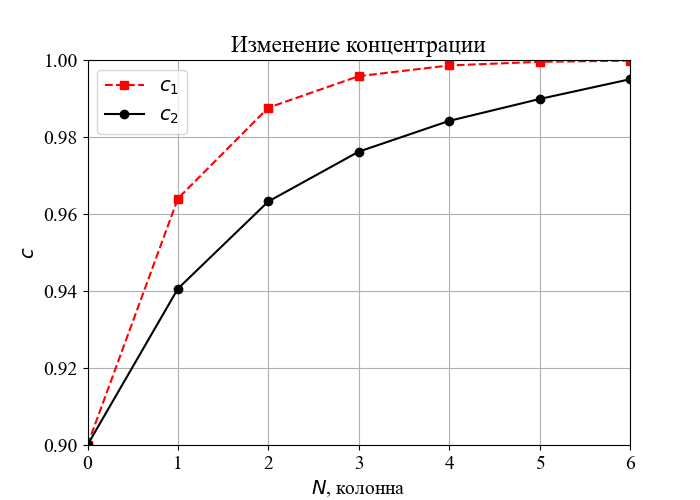
\includegraphics[scale=1]{latex/figures/concentration_change.png}
    \caption{Изменение концентрации по колоннам каскада}
    $c_{1}$ -- без отбора, $c_{2}$ -- с отбором
    \label{fig:concentraion_change}
\end{figure}

Определены величины потоков отвала и питания из уравнения материального баланса (\ref{pr:system_material}):
\begin{equation}\label{pr:system_material}
    \begin{cases}
    Fc_{F} = Pc_{P} + Wc_{W}\\
    F = P + W
    \end{cases}
\end{equation}

В данной системе уравнений неизвестными являются потоки питания ($F$) и отвала ($W$).
\begin{equation*}
    \begin{cases}
    Pc_{F} + Wc_{F} = Pc_{P} + Wc_{W}\\
    F = P + W
    \end{cases}
\end{equation*}
\begin{equation*}
    \begin{cases}
    W(c_{F} - c_{W}) = P(c_{P} - c_{F})\\
    F = P + W
    \end{cases}
\end{equation*}
\begin{equation*}
    \begin{cases}
    W = P\dfrac{c_{P} - c_{F}}{c_{F} - c_{W}}\\
    F = P + W
    \end{cases}
\end{equation*}
\begin{equation}
    W = P\dfrac{c_{P} - c_{F}}{c_{F} - c_{W}}
\end{equation}
\begin{equation}
    F = P + W
\end{equation}

$W = \var{product_flow_mol}\cdot\dfrac{\var{result_concentartion_product} - \var{concentraion_feed}}{\var{concentraion_feed} - \var{result_concentartion_waste}} \approx \var{result_waste}\text{ }\dfrac{\text{моль}}{\text{ч}}$

$F = \var{product_flow_mol} + \var{result_waste} = \var{result_feed}\text{ }\dfrac{\text{моль}}{\text{ч}}$

Принципиальная схема получившегося каскада приведена на рисунке \ref{fig:cascade_all}. Сплошными стрелками показано движение гидроксида лития, пунктиром – амальгамы.
\begin{figure}[hbtp]
    \centering
    \captionsetup{justification=centering}
    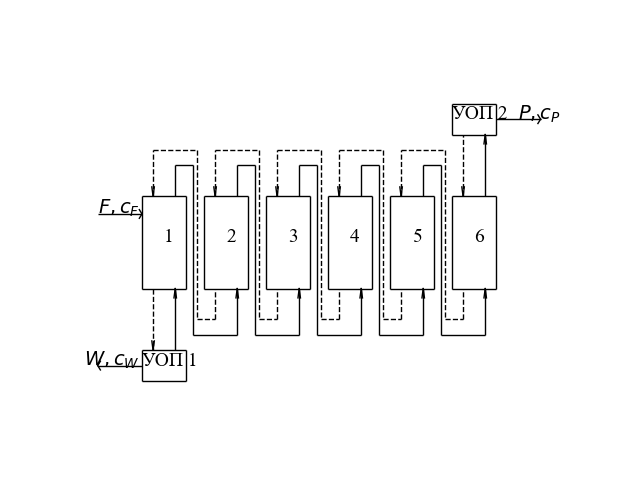
\includegraphics[scale=1]{latex/figures/cascade.png}
    \caption{Принципиальная схема каскада}
    \label{fig:cascade_all}
\end{figure}

Каскад состоит из шести колонн изотопного обмена с питанием на первой и двух узлов обращения потоков.

В узле обращения потоков 1 происходит реакция разложения амальгамы:
\begin{equation}
    Li_{n}Hg + H_{2}O \rightarrow LiOH + Hg + \dfrac{1}{2}H_{2}
\end{equation}

Образовавшийся гидроксид лития поступает в колонну изотопного обмена 1, где движется противотоком амальгаме.

В узле обращения потоков 2 протекает реакция:

\begin{equation}
    LiOH + Hg \rightarrow Li_{n}Hg + H_{2}O + \dfrac{1}{2}O_{2}
\end{equation}

Обращение проводят в электролизере с ртутным катодом \cite{mushkin}. Образовавшаяся в электролизере амальгама поступает в колонну изотопного обмена 6, где она движется противотоком к раствору.

Амальгама обогащается по легкому изотопу $^{6}$Li, раствор лития – по тяжелому $^{7}$Li.
\newpage